\section{第四章\quad 黏性流体运动及其阻力计算}

%\subsection{黏性流体运动的两种状态}

雷诺实验说明黏性流体有两种基本流态：层流状态和紊流状态，中间可出现过渡状态。\pt{小流量}时，染色液体呈清晰细线，流体质点基本不混杂，对应\pt{层流}。\pt{中流量}时，染色线开始摆动、扩散，对应\pt{过渡状态}。\pt{大流量}时，染色液体迅速扩散并与主流混合，对应\pt{紊流}。

流速增加时：$v<v_c$ 为层流；$v=v_c \to v_c'$ 时由层流进入过渡状态；$v>v_c'$ 为紊流。
流速减小时：$v=v_c' \to v_c$ 时由紊流进入过渡状态；$v<v_c$ 又恢复层流。称 $v_c'$ 为上临界速度，$v_c$ 为下临界速度。$V_c \propto \mu/(\rho d)$ \\

雷诺实验\pt{结论}：当流速大于上临界流速时为紊流；小于下临界流速时为层流；介于两者之间时，流态可能是层流也可能是紊流，取决于初始状态和外界扰动。 \\
临界雷诺数定义为 $\mathrm{Re}_c=\frac{Vd_e}{\nu}$，其中 $\nu=\frac{mu}{\rho}$。下临界雷诺数 $\mathrm{Re}_c=2300$，是流态的判别标准，只取决于流体的过水断面形状，上临界雷诺数 $\mathrm{Re}_c'=\frac{V_c'd}{\nu}$ 极易受外界扰动影响，数值不稳定，实际意义不大。

当流体流动的雷诺数 $\mathrm{Re}<\mathrm{Re}_c$ 时，流动状态为层流；当 $\mathrm{Re}>\mathrm{Re}_c$ 时，流动状态为紊流；当 $\mathrm{Re}$ 介于 $\mathrm{Re}_c$ 和 $\mathrm{Re}_c'$ 之间时，流动状态极不稳定，任意微小扰动都会破坏稳定，变为紊流。\\

工程上认为 $\mathrm{Re}le 2300$ 时为层流，$\mathrm{Re}>2300$ 为紊流。

流体在任意形状截面的管道中流动时雷诺数的形式为 $\mathrm{Re}=\frac{Vd_e}{\nu}$ 其中 $d_e=\frac{4A}{\xi}$ 为当量直径，$x$ 为湿周，指在总流的有效截面上，流体与固体壁面的接触长度。

充满流体的圆管：$d_e=d$。
边长为 $a$ 的正方形管道：$d_e=a$。
高为 $h$、宽为 $b$ 的长方形管道：$d_e=\frac{2hb}{h+b}$。
圆环形管道：$d_e=d_2-d_1$。
管束流道：$d_e=4(S_1S_2-\pi d^2/4)/(\pi d)=4S_1S_2/(\pi d)-d$。

\pt{雷诺数的物理意义}:$\mathrm{Re}=\frac{\rho Vl}{\mu}=\frac{\rho V^2 l^2}{\mu Vl}=\frac{\text{惯性力}}{\text{粘性力}}$。当 $\mathrm{Re}$ 较小时，粘性力占主导，流动状态为层流；当 $\mathrm{Re}$ 较大时，惯性力占主导，流动状态为紊流。

\pt{层流}又称片流，指流体质点不相互混杂，作有序的成层流动。\pt{特点}：有序性；黏性占主要作用；遵循牛顿内摩擦定律；能量损失与流速一次方成正比；常发生在低流速、小 $\mathrm{Re}$ 情况。\\
\pt{紊流}又称湍流，指速度、压力等物理量在时间和空间中发生不规则脉动的流体运动。\pt{特点}：无序性、随机性、有旋性、混掺性；受黏性和紊动共同作用；水头损失与流速的 $1.75 \sim 2$ 次方成正比；常发生在高流速、大 $\mathrm{Re}$ 情况。

\divider

%\subsection{管内流动阻力的两种类型}

\pt{沿程阻力}：流体与管壁面以及流体层之间存在摩擦力，流体沿路程流动时受到摩擦阻滞。\pt{沿程损失}：流体在缓变流整个流程中，为克服沿程阻力而损失的能量。

使用\pt{达西-威斯巴赫公式}计算沿程水头损失 $h_f=\lambda \frac{l}{d}\frac{V^2}{2g}$，沿程压强损失 $\Delta p_f=\lambda \frac{l}{d}\rho\frac{V^2}{2}$。
其中 $\lambda$ 为沿程阻力系数，无量纲；$l$ 为管长；$d$ 为管径；$V$ 为有效截面平均流速。

\pt{局部阻力}：流体流经阀门、弯管、变截面等局部装置时，由碰撞、旋涡等造成的阻力。\pt{局部损失}：流体在状态急剧变化的急变流中，为克服局部阻力而损失的能量。

局部水头损失通式：$h_j=\zeta \frac{\nu^2}{2g}$，对应压力损失可记为 $\Delta p_j=\zeta \rho \frac{V^2}{2}$。$\zeta$ 为局部损失系数，无量纲，一般由实验测定。

总能量损失 $h_w=\sum h_f+\sum h_j$，$\Delta p_w=\rho g h_w=\sum \Delta p_f+\sum \Delta p_j$。能量损失的量纲为长度，工程中也称为水头损失。

\divider

%\subsection{圆管内层流流动}

\pt{层流流速分布}推导：将 $\tau = -\mu \frac{\mathrm{d}\mu}{\mathrm{d}r}$ 带入沿程损失 $f_f = \frac{2\tau}{r\rho g}l$ 得到 $\mathrm{d}u = -\frac{\Delta p_f}{2\mu l}r \mathrm{d}r$ 积分得到 $u = - \frac{\Delta p_f}{4\mu l}r^2+C$ 带入边界条件得到 $C = \frac{\Delta p_f}{4\mu l }{r_0}^2$，即 $u = \frac{\Delta p_f}{4\mu l}({r_0^2}-r^2)$，$u_\text{max}=\frac{\Delta p_f}{4\mu l}{r_0}^2$，$u = u_\text{max}\left(1-\frac{r^2}{{r_0}^2}\right)$

\pt{圆管内层流流量（哈根-泊肃叶公式）}$q_v =\frac{\Delta p_f \pi}{8\mu l}{r_0}^4$，\\\pt{平均流速}$V = \frac{\Delta p_f}{8\mu l}{r_0}^2$ 为最大流速的一半\\\pt{切应力}$\tau =\frac{\Delta p_f r}{2l}$，管壁上为 $\tau _0 =\frac{\Delta p_f r_0}{2l}$，则 $\tau = \tau_0\left(\frac{r}{r_0}\right)$

\pt{圆管内层流沿程损失}$h_f = \frac{32\mu l V}{\rho g d^2}=\lambda \frac{l}{d}\frac{V^2}{2g}$ 其中 $\lambda = \frac{64}{\mathrm{Re}}$\\

\pt{动能修正系数}$\alpha = \frac{1}{A}\iint_A\left(\frac{u}{V}\right)^3\,\mathrm{d}A=\frac{1}{\pi {r_0}^2}\int_{0}^{r_0} \left\{2\left[1-\left(\frac{r}{r_0}\right)^2\right]\right\}^3\times 2\pi r \, \mathrm{d}r = 2$

\divider

%\subsection{圆管内的紊流流动}

紊流是随机的三维非定常有旋流动，判据仍以雷诺数 $\mathrm{Re}$ 为基础。\pt{脉动现象}：流动参数随时间变化的现象。\pt{时均速度}：$\bar{u}=\frac{1}{t_1}\int_0^{t_1}u,\mathrm{d}t$。\pt{脉动速度}：$u'$。瞬时速度分解：$u=\bar{u}+u'$。同理，压力和密度也可写为：$p=\bar{p}+p'$，$\rho=\bar{\rho}+\rho'$。

\pt{紊流的速度分布}：靠近壁面处，速度按近似直线规律分布，属于黏性底层。靠近管轴中心处，速度按对数规律分布，属于紊流核心区。紊流核心区速度梯度较小，速度分布较均匀；管轴线处速度最大，因为紊流中质点脉动掺混强烈，动量交换明显。

\par\vspace{0.5pt}
{\centering
    \renewcommand{\arraystretch}{1.6}
    \resizebox{\linewidth}{!}{%
        \begin{tabular}{c|c|c|c|c|c}
            \hline
            $\boldsymbol{Re}$
             & $\mathbf{4.0\times10^3}$
             & $\mathbf{2.3\times10^4}$
             & $\mathbf{1.1\times10^5}$
             & $\mathbf{1.1\times10^6}$
             & $\mathbf{(2.0\sim3.2)\times10^6}$ \\
            \hline
            $\boldsymbol{V'/u_{\max}}$
             & $\mathbf{0.7912}$
             & $\mathbf{0.8073}$
             & $\mathbf{0.8167}$
             & $\mathbf{0.8497}$
             & $\mathbf{0.8658}$                 \\
            \hline
        \end{tabular}%
    }
    \par}

\pt{紊流结构分区}：黏性底层区，也称层流底层；层流向紊流的过渡区；充分发展紊流区，也称紊流核区。流速越高，$\mathrm{Re}$ 越大，层流底层越薄。
绝对粗糙度 $\Delta$：管壁粗糙凸出部分的平均高度。相对粗糙度：$\Delta/d$。

\pt{水力光滑管的紊流区} $\delta=\frac{58.3d}{\mathrm{Re}^{0.875}}$，适用于 $4\times 10^3<\mathrm{Re}<10^5$\\
\pt{一般的形式} $\delta=\frac{32.8d}{\mathrm{Re}\sqrt{\lambda}}$，适用于已知沿程阻力系数 $\lambda$ 时。

若黏性底层厚度 $\delta>\Delta$，粗糙凸起被黏性底层淹没，管道表现为水力光滑管。若 $\delta<\Delta$，粗糙凸起伸出黏性底层，管道表现为水力粗糙管。同一根管道在不同流速下，可能表现为光滑管，也可能表现为粗糙管。

\pt{紊流的切向应力}:摩擦切向应力：由流体黏性和相邻流层时均速度差引起$\tau_v=\mu\frac{\mathrm{d}u}{\mathrm{d}y}$。
附加切向应力：由横向脉动速度、质点掺混和动量交换引起 $\tau_t\propto \left(\frac{\mathrm{d}u}{\mathrm{d}y}\right)^2$。 紊流总切应力：$\tau=\tau_v+\tau_t$。接近管壁处，$\tau_v$ 起主要作用，$\tau_t$ 可略去。管道中心处，质点混杂强烈，$\tau_t$ 起主要作用，$\tau_v$ 可略去。管壁切应力：$\tau_0=\frac{\Delta p r_0}{2l}$。流管表面切应力：$\tau=\frac{\Delta p r}{2l}$。有效截面上的切应力分布：$\tau=\tau_0\frac{r}{r_0}$。层流与紊流虽然切应力沿半径都呈线性分布形式，但 $\tau_0$ 不同，所以分布斜率不同。在层流底层中，摩擦切应力占主要地位。

在紊流核心中附加切应力占主要地位紊流沿程损失仍采用达西-威斯巴赫形式：$h_f=\lambda\frac{l}{d}\frac{V^2}{2g}$。紊流计算的关键是确定沿程阻力系数 $\lambda$。紊流中 $\lambda=f(\mathrm{Re},\Delta/d)$，即同时与雷诺数和相对粗糙度有关。

\divider

%\subsection{圆管流动的沿程损失系数的确定}

\pt{尼古拉兹实验}：研究不同雷诺数和不同粗糙度下圆管沿程阻力系数 $\lambda$ 的变化规律。将黄沙筛分成由细到粗六种颗粒，分别粘贴在光滑管内壁上，形成不同人工粗糙度。采用三种不同管径：$25,\mathrm{mm}$、$50,\mathrm{mm}$、$100,\mathrm{mm}$。采用六种不同粗糙度，以通过改变流量改变 $\mathrm{Re}$。测出沿程损失 $h_f$，再由 $h_f=\lambda\frac{l}{d}\frac{V^2}{2g}$ 反求 $\lambda$。 $r/\Delta$ 表示，数值为 $15$、$30.6$、$60$、$126$、$252$、$507$。

\noindent
\begin{minipage}[t]{0.64\linewidth}
    \vspace{0pt}
    \raggedright
    $\MRN{1}$ 层流区：$\mathrm{Re}<2300$，有 $\lambda=\frac{64}{\mathrm{Re}}$。\\
    $\MRN{2}$  过渡区：$2300<\mathrm{Re}<4000$，情况复杂，无一定规律。\\
    $\MRN{3}$  紊流水力光滑管区： $4000<\mathrm{Re}<59.6(r/\Delta)^{8/7}$。满足布拉修斯公式，$\lambda = \frac{0.3164}{\mathrm{Re}^{0.25}}$。$10^5 <\mathrm{Re}<3\times 10^6$满足尼古拉兹经验公式 $\frac{1}{\sqrt{\lambda}}= 2.0\lg(\mathrm{Re}\sqrt{\lambda})-0.8$\\
\end{minipage}
\hfill
\begin{minipage}[t]{0.35\linewidth}
    \vspace{0pt}
    \centering
    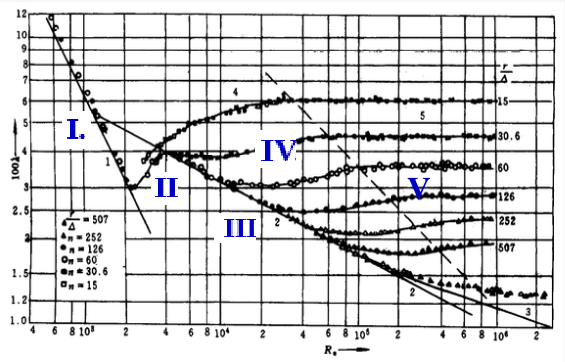
\includegraphics[width=\linewidth]{figures/4尼古拉兹实验曲线图.png}
\end{minipage}

$\MRN{4}$ 紊流水力粗糙管过渡区：$59.6(r/\Delta)^{8/7}<\mathrm{Re}<4160(r/\Delta)^{0.85}$。可使用洛巴耶夫公式 $$\lambda=1.42[\lg(\mathrm{Re}d/\Delta)]^{-2}=1.42[\lg(1.273q_V/(\nu\Delta))]^{-2}$$ 或者科尔布鲁克公式 $\frac{1}{\sqrt{\lambda}}=-2\lg\left(\frac{2.51}{\mathrm{Re}\sqrt{\lambda}}+\frac{\Delta/d}{3.7}\right)$ \\
$\MRN{5}$ 紊流水力粗糙管平方阻力区：$\mathrm{Re}>4160(r/\Delta)^{0.85}$，满足尼古拉兹经验公式 $\frac{1}{\sqrt{\lambda}}=2\lg\frac{d}{2\Delta}+1.74$

实验意义：紊流复杂，管壁粗糙度会影响 $\lambda$，无法像层流那样完全由理论推出。需要通过实验测定并归纳出经验公式。尼古拉兹实验是系统性强、参数范围广的代表性实验。实验局限：实验采用人工粗糙度，与工业管道自然粗糙度差异较大，不能直接完全套用。

\noindent
\begin{minipage}[t]{0.48\linewidth}
    \vspace{0pt}
    \raggedright
    \pt{莫迪图}\\
    适用范围为 $600<\mathrm{Re}<10^8$ 用图时通常根据 $ \mathrm{Re} $ 和 $ \Delta/d $ 查取 $ \lambda $。与尼古拉兹曲线相比，莫迪图更适合工程管道实际计算
\end{minipage}
\hfill
\begin{minipage}[t]{0.48\linewidth}
    \vspace{0pt}
    \centering
    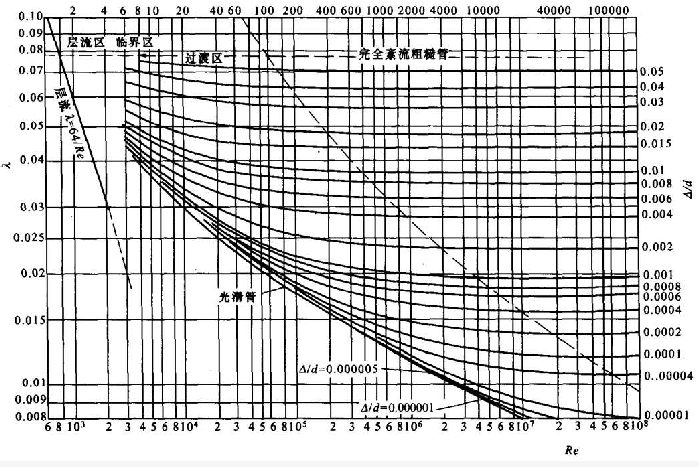
\includegraphics[width=\linewidth]{figures/4莫迪图.png}
\end{minipage}

\divider

%\subsection{局部损失计算}

局部损失产生位置：阀门、弯管、突然扩大、突然缩小等管件处。流通截面或流动方向急剧变化，引起速度场迅速改变，增加流体间摩擦、碰撞并形成旋涡，从而产生局部损失

$h_j = \frac{({V_1}^2-{V_2}^2)}{2g}=\frac{V_1^2}{2g}\left(1-\frac{A_1}{A_2}\right)^2=\frac{V_2^2}{2g}\left(\frac{A_2}{A_1}-1\right)^2$，$\zeta_1=\left(1-\frac{A_1}{A_2}\right)^2$，$\zeta_2=\left(\frac{A_2}{A_1}-1\right)^2$，则局部损失可写成 $h_j=\zeta_1\frac{V_1^2}{2g}=\zeta_2\frac{V_2^2}{2g}$。\\

\par\vspace{0.5pt}
{\centering
    \renewcommand{\arraystretch}{1.45}
    \resizebox{\linewidth}{!}{%
        \begin{tabular}{c|c|c|c|c|c|c|c|c|c|c|c}
            \hline
            $\frac{A_1}{A_2}=\left(\frac{d_1}{d_2}\right)^2$
             & $\mathbf{0}$
             & $\mathbf{0.1}$
             & $\mathbf{0.2}$
             & $\mathbf{0.3}$
             & $\mathbf{0.4}$
             & $\mathbf{0.5}$
             & $\mathbf{0.6}$
             & $\mathbf{0.7}$
             & $\mathbf{0.8}$
             & $\mathbf{0.9}$
             & $\mathbf{1.0}$ \\
            \hline
            $\zeta_1$
             & $1.0$
             & $0.81$
             & $0.64$
             & $0.5$
             & $0.36$
             & $0.25$
             & $0.16$
             & $0.09$
             & $0.04$
             & $0.01$
             & $0$            \\
            \hline
            $\zeta_2$
             & $\infty$
             & $81$
             & $16$
             & $5.44$
             & $2.25$
             & $1.0$
             & $0.444$
             & $0.184$
             & $0.0625$
             & $0.0123$
             & $0$            \\
            \hline
        \end{tabular}%
    }
    \par}

突然扩大 $A_2\gg A_1$，$\zeta_1 \approx 1,\zeta_2 \approx \infty$，突然缩小有经验公式 $\zeta_2 =0.5 \left(1-\frac{A_2}{A_1}\right)$ $A_1\gg A_2$，$\zeta_2 \approx 0.5$。\\

\divider

%\subsection{管道水力计算}

\pt{管道系统分类}
\begin{itemize}
    \item \pt{按照能量损失大小分类}：长管：局部阻力在总阻力中的比例不足 $5\%$ 的管道系统，称为水力长管，计算时只考虑沿程损失；短管：水力计算中需要同时考虑沿程损失和局部损失的管道系统。
    \item \pt{按照管道系统结构}：简单管道：管径和粗糙度均相同的一根或数根管子串联而成；复杂管道：包括串联管道、并联管道、枝状管道、网状管道。
\end{itemize}

管道系统分类类似电路系统，水力计算类似电路计算。将管道中的流量比作电流，压降比作电压降\\

\pt{串联管道}：串联管道中各段的流量相等，对于不可压缩流体 $q*{V1}=q*{V2}=q_{V3}=\cdots=\mathrm{const}$，$V_1A_1=V_2A_2=V_3A_3=\cdots=\mathrm{const}$。总能量损失是各段管道中的能量损失之和 $h_w = h_{w1}+h_{w2}+h_{w3}+\cdots$，若各管段的管径相同，称为简单管道，则各管段的平均流速也相等

\pt{并联管道}：对于不可压缩流体 $q_V = q_{V1}+q_{V2}+q_{V3}+\cdots$，两点之间的能量损失相同，为这两节点之间的压头差 $h_{W1}=h_{w2}=h_{w3}=h_{w(a-b)}$

\pt{基本公式}：\\
\pt{连续性方程}：$q_m=\rho_1gV_1A_1=\rho_2gV_2A_2=\mathrm{const}$ 或者 $q_V = V_1A_1=V_2A_2 =\mathrm{const}$\\
\pt{伯努利方程}:$z_1+\frac{p_1}{\rho g}+\frac{{V_1}^2}{2g}=z_2+ \frac{p_2}{\rho g}+h_2$\\
\pt{能量损失}:$h_w = \sum h_f +\sum h_j$, $h_f=\lambda \frac{l}{d}\frac{V^2}{2g}$,$h_j=\zeta \frac{V^2}{2g}$

\divider
